% Student template

\clearpage
\checkoddpage

\sectionmark{Steckbrief - \stdname}

% Returns a default file if not found
\providecommand\dfincludegraphics[2][]{
	\IfFileExists{#2}
	{
		\includegraphics[#1]{#2}
	}
	{
		%\fbox{File not found}
	}
}

% Ring
\def\ringx{50pt}
\def\ringy{250pt}
\def\ringwidth{250pt}
\def\ringimgwidth{180pt}
\def\ringoffset{(\ringwidth - \ringimgwidth) / 2}
\ifoddpage\else
	\def\ringx{-\paperwidth - 350pt} % ringwidth + 2 * ringx
\fi
\AddToShipoutPictureBG*{
	\AtTextUpperLeft{
		\put(-\ringx + \ringoffset, -\ringy + \ringoffset){
			\dfincludegraphics[keepaspectratio=true, width=\ringimgwidth]{parts/students/figures/bornerma.jpg}
		}
		\put(-\ringx, -\ringy){
			\oddflip[keepaspectratio=true, width=\ringwidth]{ring.png}
		}
	}
}

% Frame
\def\framex{130pt}
\def\framey{20pt}
\def\framewidth{180pt}
\def\frameimgwidth{160pt}
\def\frameoffset{(\framewidth - \frameimgwidth) / 2}
\ifoddpage\else
	\def\framex{518pt} % paperwidth - framewidth / 2
\fi
\AddToShipoutPictureBG*{
	\AtTextLowerLeft{
		\put(\textwidth - \framex + \frameoffset, \framey + \frameoffset + 8pt){
			\dfincludegraphics[keepaspectratio=true, width=\frameimgwidth]{parts/students/figures/child_\stdid.jpg}
		}
		\put(\textwidth - \framex, \framey){
			\oddflip[keepaspectratio=true, width=\framewidth]{rahmen.png}
		}
	}
}

% Steckbrief Tabelle
\ifoddpage
	\def\tablex{0.5\linewidth}
\else
	\def\tablex{-1cm}
\fi
\def\tablewidth{0.6\linewidth}

\hspace*{\tablex}\Large\begin{minipage}{\tablewidth}
	\begin{tabular}{@{}ll@{}}
		\textbf{Name:}          & \stdname                                                  \\
		\textbf{Geburtstag:}    & \multicolumn{1}{p{\tablewidth}}{\RaggedRight\stdbirthday} \\
		\textbf{Lieblingsfach:} & \multicolumn{1}{p{\tablewidth}}{\RaggedRight\stdfavsub}   \\
		\textbf{Hassfach:}      & \multicolumn{1}{p{\tablewidth}}{\RaggedRight\stdhatesub}  \\
		\textbf{Hobbies:}       & \multicolumn{1}{p{\tablewidth}}{\RaggedRight\stdhobbies}  \\
		\textbf{Musik:}         & \multicolumn{1}{p{\tablewidth}}{\RaggedRight\stdmusic}    \\
	\end{tabular}\\~\\
	\textbf{Das werde ich am meisten vermissen:}\\\stdmissing\\~\\
	\textbf{Ohne das hätte ich die Oberstufe nicht geschafft:}\\\stdmotivation\\~\\
	\textbf{Lebensmotto:}\\\stdquote\\~\\
	\textbf{Zukunftspläne:}\\\stdfuture\\~\\
	%\textbf{Erkennungsmerkmale:}\\\stdidk\\~\\
\end{minipage}

\begin{figure}[H]
	\hspace*{-2.5cm}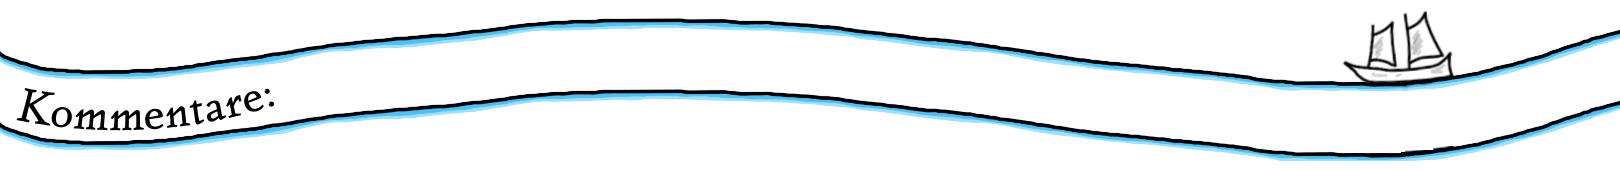
\includegraphics[keepaspectratio=true, width=\paperwidth]{mittelwelle.png}
\end{figure}
